\documentclass[10pt,letterpaper,final]{article}
\usepackage[left=4cm,rigth=4cm,top=4cm,bottom=2cm]{geometry}
\usepackage[utf8]{inputenc}
\usepackage{amsmath}
\usepackage{amsfonts}
\usepackage{amssymb}
\usepackage{graphicx}
\usepackage{kpfonts}
\usepackage{tabularx}
\usepackage{hyperref}
\usepackage{natbib}

%\newcommand{\X}{\multicolumn{1}{|c|}{$\times$}}


\begin{document}
    \section*{}
    \title{Sistema de Detección y Evasión de Colisiones basado en Visión Computacional para Vehículos Autónomos}
    \author{Rubén Martínez González}
    \maketitle
    \clearpage
    \section*{Introducción}
    \noindent
    El avance continuo en la tecnología de vehículos autónomos representa un logro significativo en la revolución del transporte.
    Existe la necesidad de desarrollar sistemas ``inteligentes'' que permitan a estos vehículos aprender a conducir de manera autónoma y,
    al mismo tiempo, detectar posibles colisiones y reaccionar de manera similar a como lo haría un conductor humano.
    La convergencia de la inteligencia artificial, la visión computacional y los sistemas de control ha generado una nueva era en la movilidad,
    desafiando y redefiniendo las fronteras de la conducción convencional.\\ \newline
    En este contexto, este trabajo se centra en el desarrollo de un sistema de detección y evasión de colisiones basado en visión computacional.
    Si bien los avances en la conducción autónoma han sido significativos, la detección y respuesta a
    situaciones de peligro, como colisiones inminentes, siguen siendo un desafío complejo.\\ \newline
    La seguridad en la carretera y la confianza del público en esta tecnología dependen en gran medida de la capacidad
    de los vehículos autónomos para enfrentar situaciones de tráfico de manera eficiente y segura.\\ \newline
    Esta investigación busca abordar esta problemática crítica, avanzando hacia un futuro en el que los vehículos autónomos
    sean capaces de igualar e incluso superar las habilidades de conducción humana en términos de detección y respuesta
    a situaciones de colisión.
    \clearpage
    
    \section*{Contexto y problemática}
    \noindent En la constante evolución de la movilidad, los vehículos autónomos representan una innovación trascendental.
    No obstante, el desafío primordial reside en dotar a estos vehículos con la capacidad de identificar y reaccionar ante situaciones de riesgo
    de manera precisa y oportuna. La detección temprana de posibles colisiones, amenazas viales y transgresiones graves a las normativas de tráfico
    es un aspecto esencial para garantizar la seguridad y la eficacia de estos sistemas autónomos. La visión computacional,
    utilizando las cámaras de video y sensores, se presenta como una estrategia central para esta detección,
    pero aún persisten desafíos tecnológicos significativos en la identificación y procesamiento oportuno de dichos eventos.
    \section*{Objetivos}
    \noindent{Objetivo general:}
    \newline
    \noindent Implementar un sistema de detección y evasión de colisiones basado en visión computacional para vehículos autónomos,
    \newline
    \newline
    \noindent{Objetivos específicos:}
    \begin{itemize}
        \item Modelar un ambiente de simulación donde un vehiculo circule por calles transitadas.
        \item Obtener datos de los sensores del vehiculo en simulación.
        \item Interpretar los datos de los sensores mediante técnicas de visión computacional.
        \item Procesar los datos y aprender a reaccionar.
    \end{itemize}
    \clearpage
    \section*{Estado del arte - Trabajos previos relacionados}
    \newline
    \begin{longtable}
        \hline
        \noindent \textbf{Referencia:}~\cite{bachute2021autonomous}                                    \\
        \textbf{Título:}                                                                               \\
        Autonomous Driving Architectures: Insights of Machine Learning and Deep Learning Algorithms \\
        \textbf{Autores:}                                                                              \\
        Bachute, Mrinal R and Subhedar, Javed M                                                        \\
        \textbf{Año:}                                                                                  \\
        2021                                                                                           \\
        \textbf{Revista:}
        Machine Learning with Applications                                                             \\
        \textbf{URL:}
        \url{https://www.sciencedirect.com/science/article/pii/S2666827021000827}                      \\
        \textbf{Resumen:}
        \begin{itemize}
            \item El artículo ofrece una visión general de cómo se aplican algoritmos de Aprendizaje Automático y Aprendizaje
            Profundo en sistemas de conducción autónoma y se enfoca en la evaluación de su desempeño en diversas tareas clave.
            \item Se centra en la investigación en el campo de la conducción autónoma y destaca que esta área está ganando
            impulso debido a las ventajas inherentes de los sistemas de conducción autónoma.
            \item Ventajas de la conducción autónoma, como la reducción de la intervención humana y la disociación del conductor del vehículo.
            \item La complejidad de los sistemas de conducción autónoma, que involucra la integración de múltiples subsistemas.
            \item Se analizan diversas tareas en la conducción autónoma, incluyendo la planificación de movimiento, la localización del vehículo,
            la detección de peatones, la detección de señales de tráfico, la detección de marcas viales, el estacionamiento automatizado,
            la ciberseguridad del vehículo y el diagnóstico de fallas del sistema.
            \item Uso de algoritmos de Aprendizaje Automático y Aprendizaje Profundo en arquitecturas de conducción autónoma para realizar estas tareas.
            \item Evaluación y comparación de algoritmos basada en métricas.
        \end{itemize}
        
        \begin{figure}[!ht]
            \begin{subfigure}
                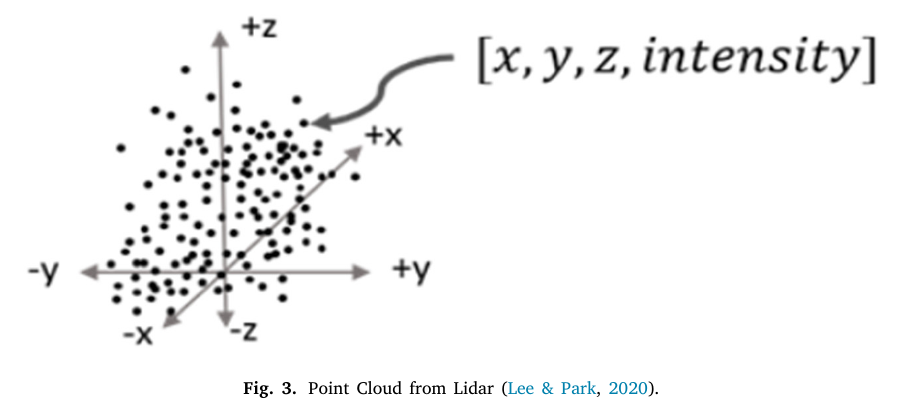
\includegraphics[width=0.5\textwidth]{img/1- Screenshot_20231106_142913}\label{fig:11}
            \end{subfigure}
            \begin{subfigure}
                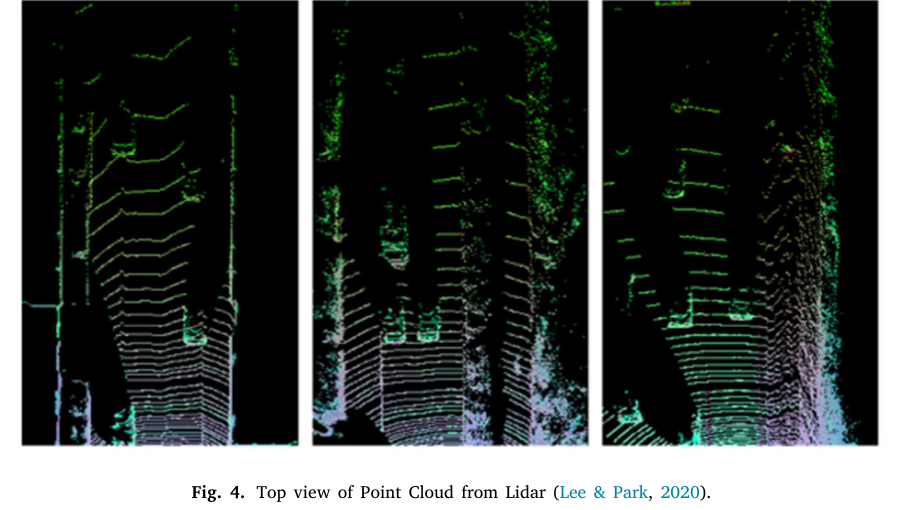
\includegraphics[width=0.5\textwidth]{img/12Screenshot_20231106_142954}\label{fig:12}
            \end{subfigure}
            \begin{subfigure}
                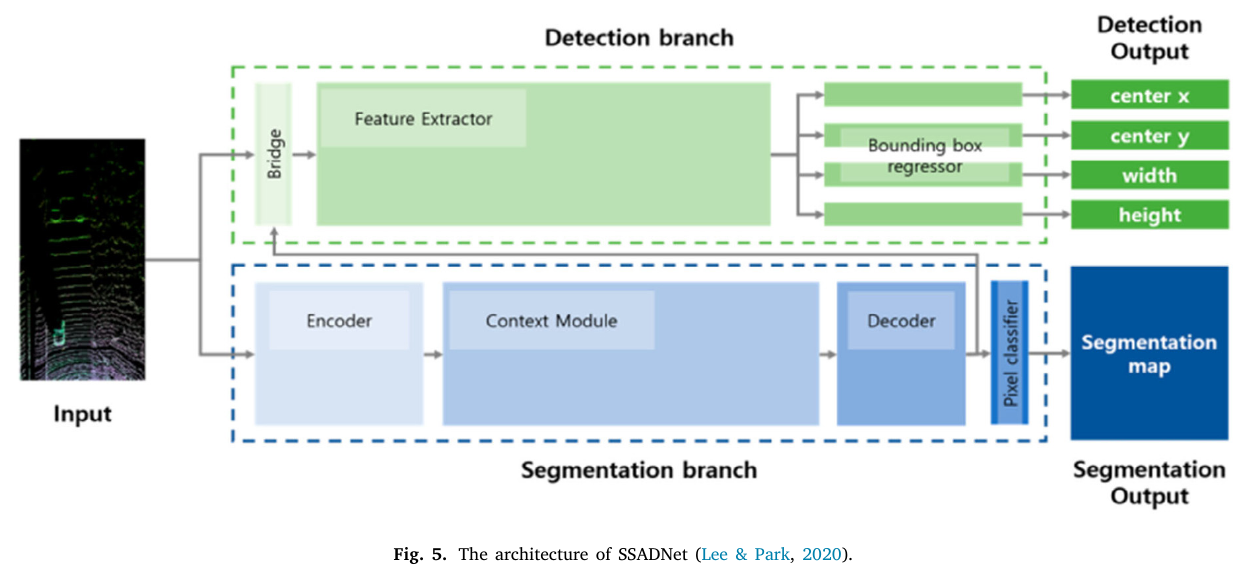
\includegraphics[width=0.6\textwidth]{img/13Screenshot_20231106_143018}\label{fig:13}
            \end{subfigure}
            \begin{subfigure}
                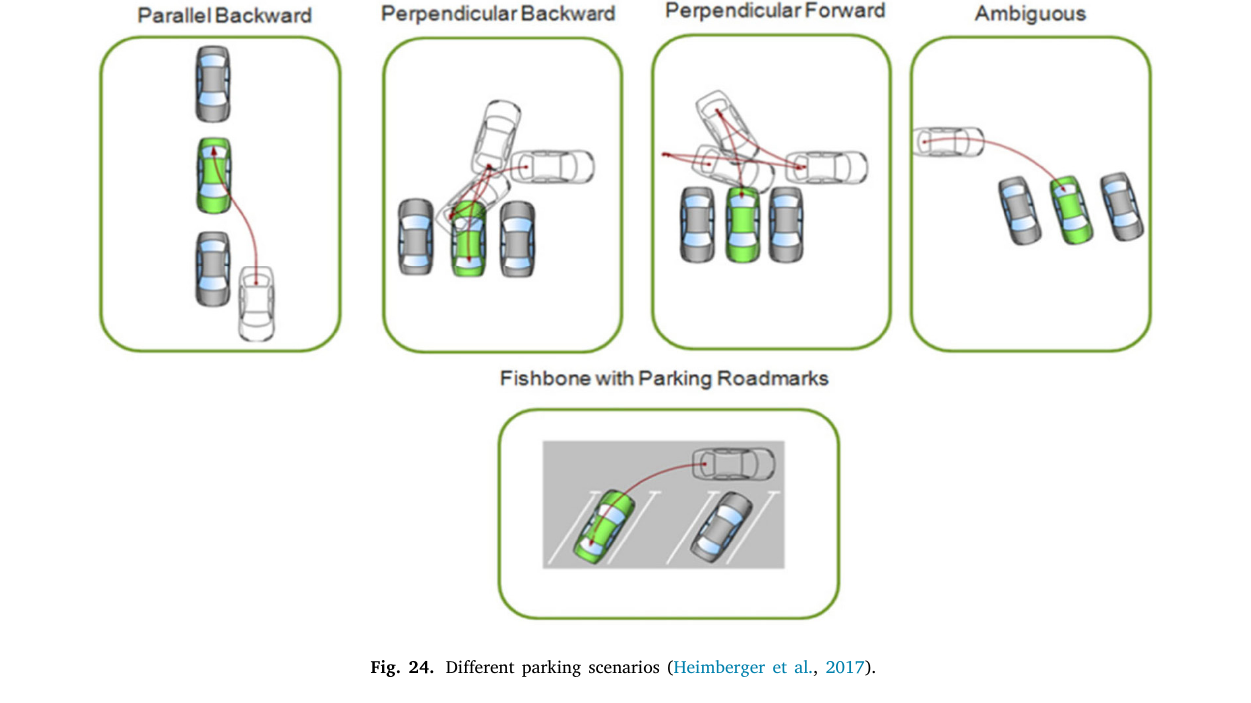
\includegraphics[width=0.6\textwidth]{img/15Screenshot_20231106_143633}\label{fig:15}
            \end{subfigure}
            \begin{subfigure}
                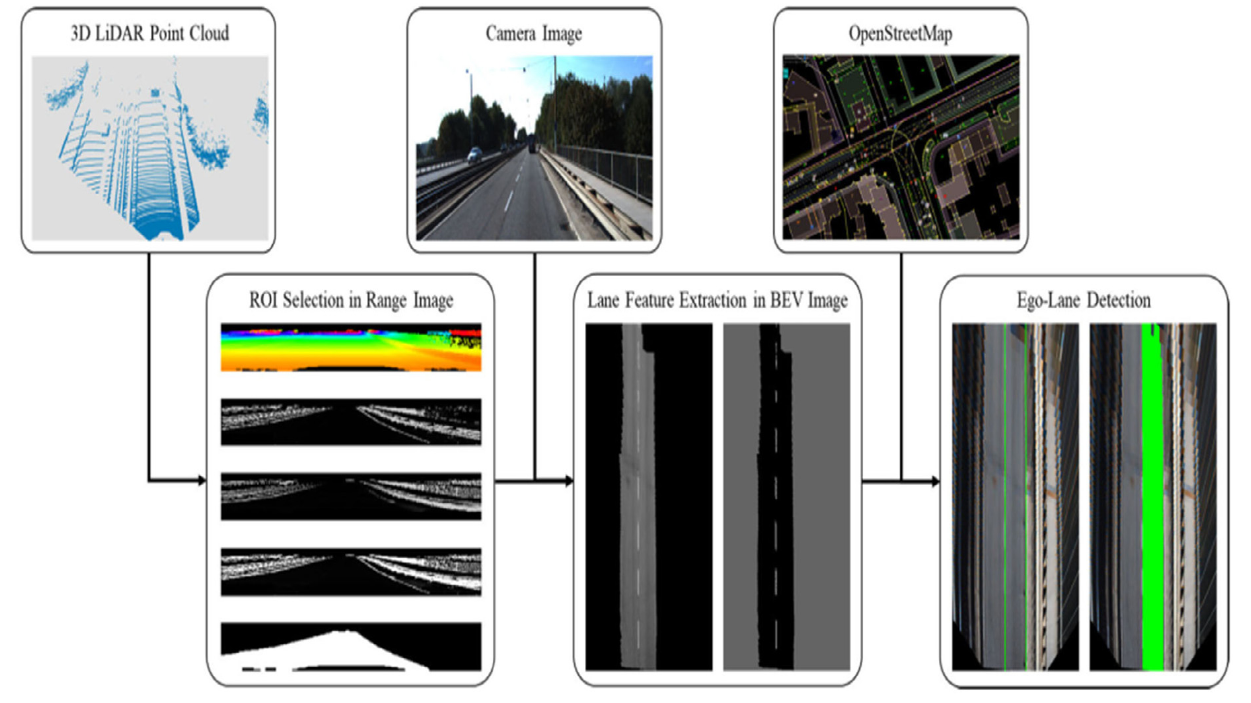
\includegraphics[width=0.9\textwidth]{img/14 Screenshot_20231106_143419}\label{fig:14}
            \end{subfigure}
            \begin{subfigure}
                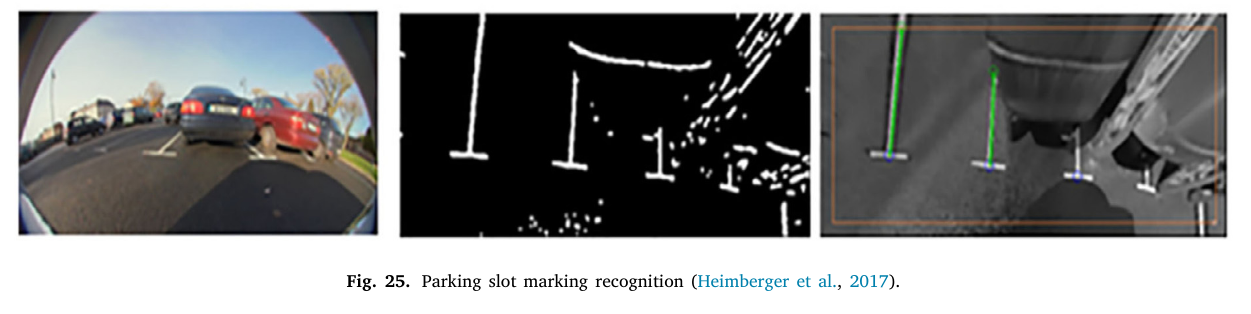
\includegraphics[width=0.8\textwidth]{img/16Screenshot_20231106_143701}\label{fig:16}
            \end{subfigure}
        \end{figure}
        \clearpage
        
        \hline
        \noindent \textbf{Referencia:}~\cite{cai2021vision}                                            \\
        \textbf{Título:}                                                                               \\
        Vision-based autonomous car racing using deep imitative reinforcement learning                 \\
        \textbf{Autores:}
        Cai, Peide and Wang, Hengli and Huang, Huaiyang and Liu, Yuxuan and Liu                        \\
        \textbf{Año:}
        2021                                                                                           \\
        \textbf{Revista:}
        IEEE Robotics and Automation Letters                                                           \\
        \textbf{URL:}
        \url{https://ieeexplore.ieee.org/abstract/document/9488179}                                    \\
        \textbf{Resumen:}
        \begin{itemize}
            \item El automovilismo autónomo es un desafío en el campo del control robótico, que históricamente ha requerido mapas precisos,
            localización y planificación, lo que lo hace computacionalmente ineficiente y sensible a cambios en el entorno.
            \item Recientemente, se han desarrollado sistemas de aprendizaje profundo de extremo a extremo que muestran resultados prometedores
            en la conducción/racing autónoma.Sin embargo, estos sistemas suelen basarse en aprendizaje por imitación supervisada (IL),
            que enfrenta problemas de discrepancia en la distribución de datos.
            \item También se han utilizado métodos de aprendizaje por refuerzo (RL), pero requieren una gran cantidad de datos de interacción riesgosa.
            \item se presenta un enfoque general de aprendizaje profundo imitativo y de refuerzo (DIRL) que logra el automovilismo
            autónomo ágil utilizando entradas visuales.
            \item El conocimiento de conducción se adquiere tanto del aprendizaje por imitación como del aprendizaje basado en modelos de RL,
            permitiendo al agente aprender de instructores humanos y mejorar su rendimiento interactuando con un modelo de mundo offline.
            \item Se valida el algoritmo en una simulación de conducción de alta fidelidad y en un automóvil RC a escala 1/20
            en el mundo real con capacidad computacional limitada.
            \item Los resultados de la evaluación muestran que el método supera a los enfoques anteriores de IL y RL en eficiencia
            de muestra y rendimiento en la tarea.
        \end{itemize}                                                                                  \\
        \begin{figure}[!ht]
            \begin{subfigure}
                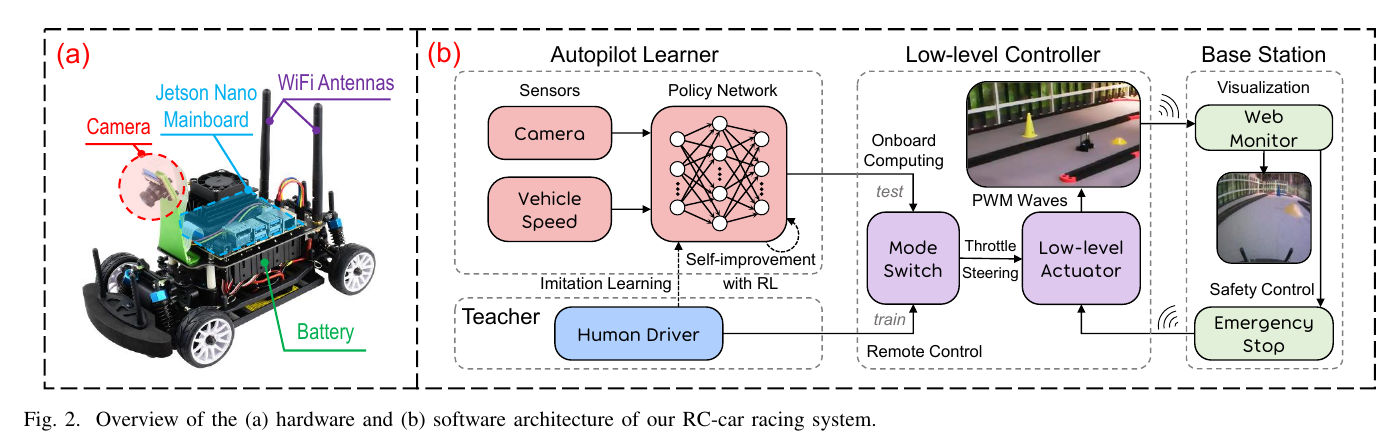
\includegraphics[width=\textwidth]{img/21}\label{fig:21}
            \end{subfigure}
            \begin{subfigure}
                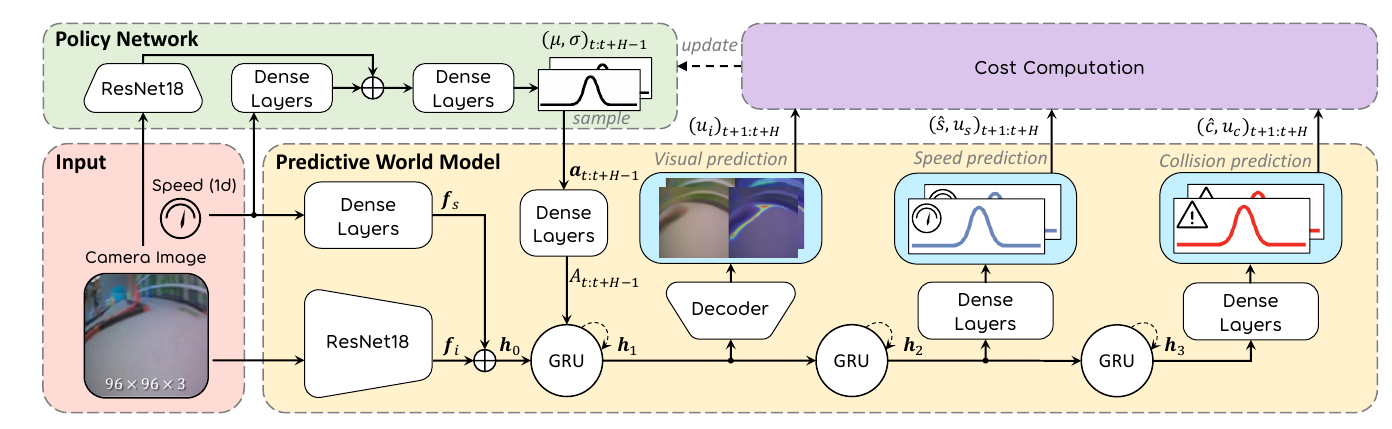
\includegraphics[width=\textwidth]{img/22}\label{fig:22}
            \end{subfigure}
            \begin{subfigure}
                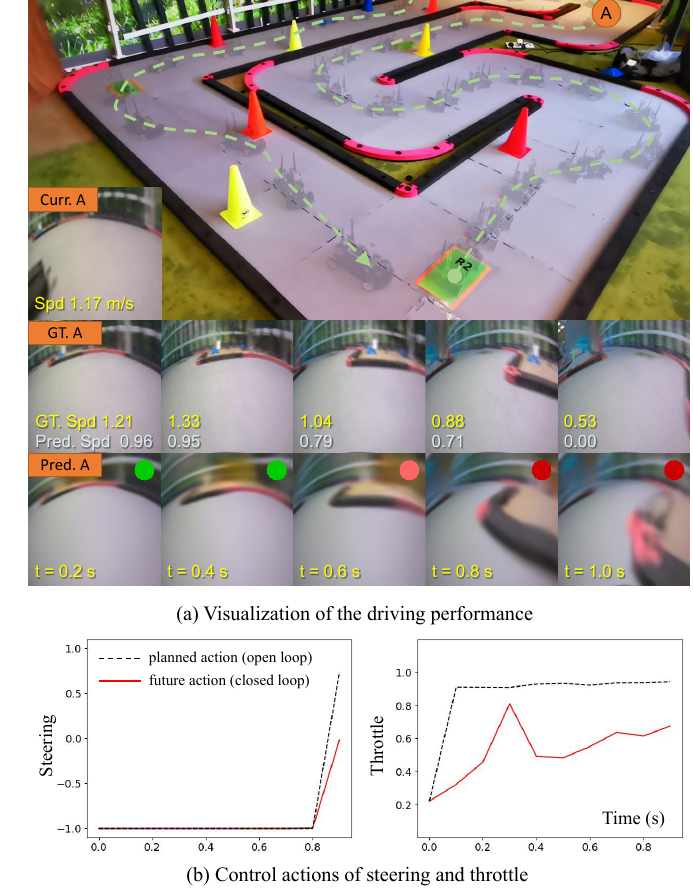
\includegraphics[width=0.6\textwidth]{img/23}\label{fig:23}
            \end{subfigure}
        \end{figure}

%        \begin{minipage}{0.5\textwidth}
%            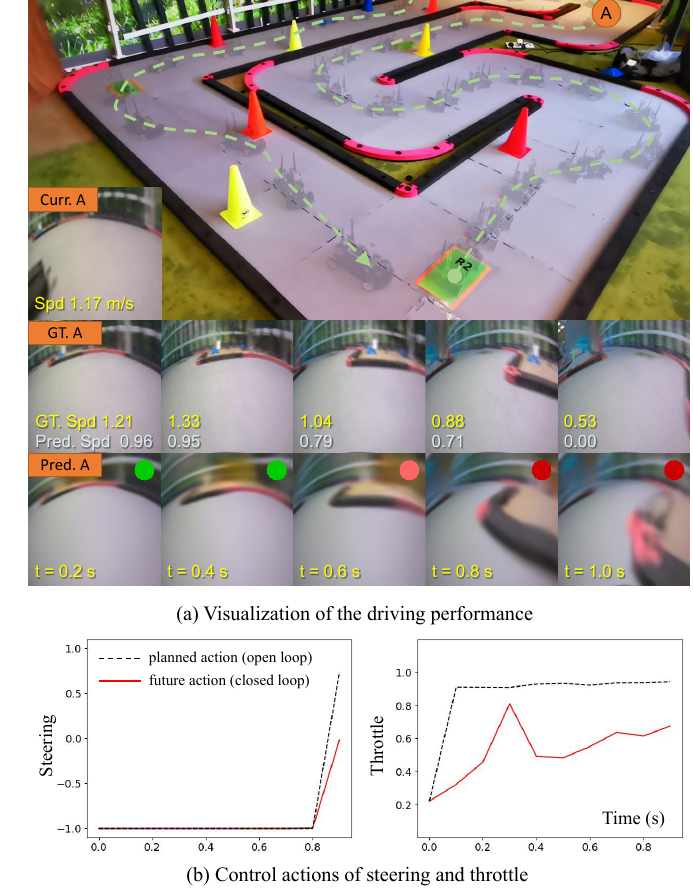
\includegraphics[width=\textwidth]{img/23}
%        \end{minipage}
%        \begin{minipage}{0.5\textwidth}
%            Rendimiento de conducción del coche.\\
%            (a) Se toma el punto A en la trayectoria para el análisis y los relacionados
%            Los ensueños se muestran en la fila inferior con imágenes futuras reales para
%            comparación. Tenga en cuenta que los ensueños no se obtienen durante las pruebas, sino que son posteriores.
%            renderizado con observaciones actuales y acciones de bucle abierto.\\
%            (b) El planificado acciones de circuito abierto (planificadas por la red de políticas en cada paso, pero solo el
%            se ejecutará el primero) en el punto A y acciones de bucle cerrado relacionadas (el
%            acciones realmente ejecutadas registradas por el coche).
%        \end{minipage}
        
        \clearpage
        \hline
        \noindent \textbf{Referencia:}~\cite{althoff2009model}                                         \\
        \textbf{Título:}                                                                               \\
        Model-based probabilistic collision detection in autonomous driving                            \\
        \textbf{Autores:}
        Althoff, Matthias and Stursberg, Olaf and Buss                                                 \\
        \textbf{Año:}
        2009                                                                                           \\
        \textbf{Revista:}
        IEEE Transactions on Intelligent Transportation Systems                                        \\
        \textbf{URL:}
        \url{https://ieeexplore.ieee.org/abstract/document/4895669}                                    \\
        \textbf{Resumen:}                                                                              \\
        \begin{itemize}
            \item El artículo se centra en la seguridad de los caminos planificados para autos autónomos en relación con otros participantes en el tráfico.
            \item Se predice la ocupación de la carretera por otros vehículos de manera estocástica.
            \item La predicción tiene en cuenta las incertidumbres derivadas de las mediciones y los posibles comportamientos
            de los otros participantes en el tráfico.
            \item También se considera la interacción entre los participantes en el tráfico y las limitaciones de las maniobras
            de conducción debido a la geometría de la carretera.
            \item El resultado principal del enfoque presentado es la probabilidad de que ocurra un choque para una trayectoria específica de un auto autónomo.
            \item El enfoque se destaca por su eficiencia, ya que la mayoría de los cálculos intensivos se realizan de manera
            offline, lo que permite disponer de un algoritmo en línea eficiente para aplicaciones en tiempo real.
        \end{itemize}                                                                                  \\
        \begin{figure}[!ht]
            \begin{subfigure}
                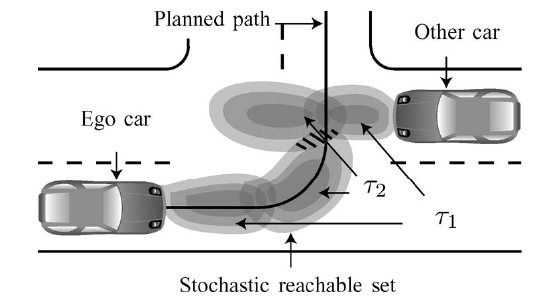
\includegraphics[width=0.5\textwidth]{img/31}\label{fig:31}
            \end{subfigure}
            \begin{subfigure}
                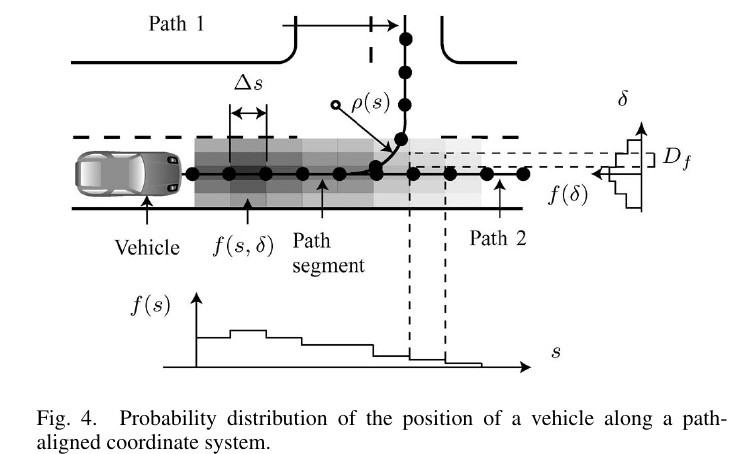
\includegraphics[width=0.5\textwidth]{img/32}\label{fig:32}
            \end{subfigure}
            \vspace{2cm}
            \begin{subfigure}
                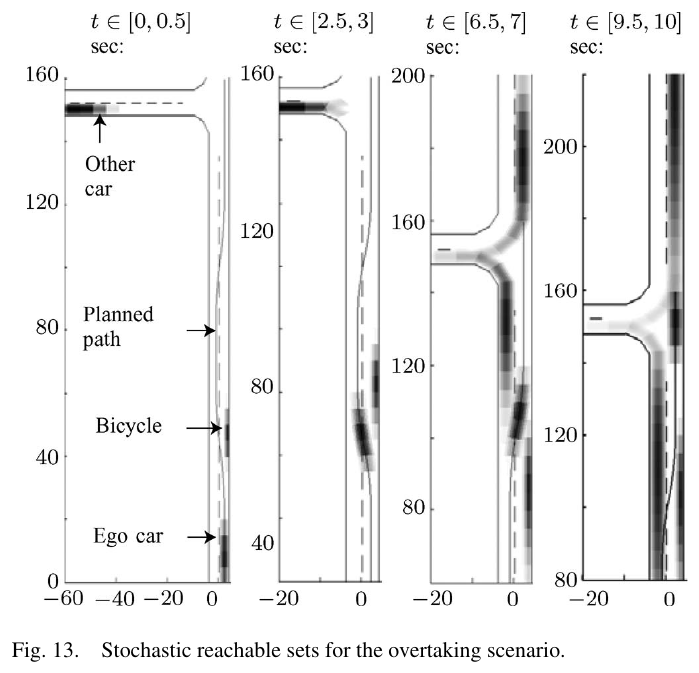
\includegraphics[width=0.5\textwidth]{img/33}\label{fig:33}
            \end{subfigure}
            \begin{subfigure}
                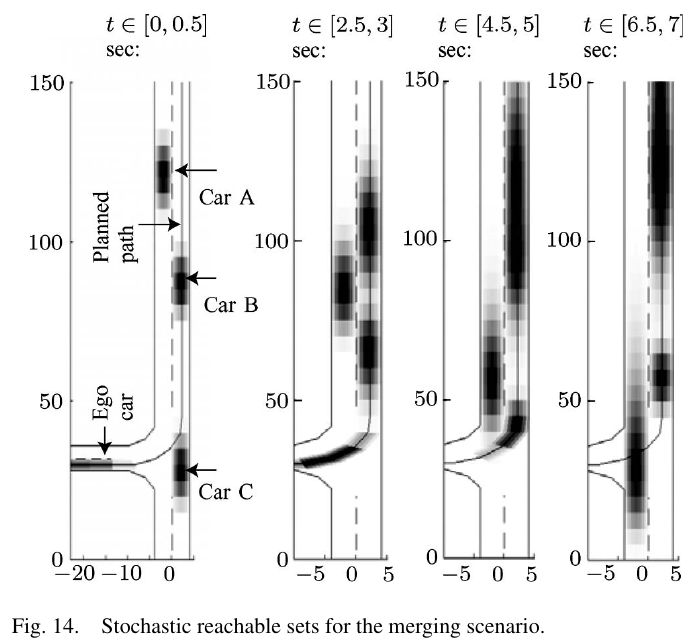
\includegraphics[width=0.5\textwidth]{img/34}\label{fig:34}
            \end{subfigure}
            \begin{subfigure}
                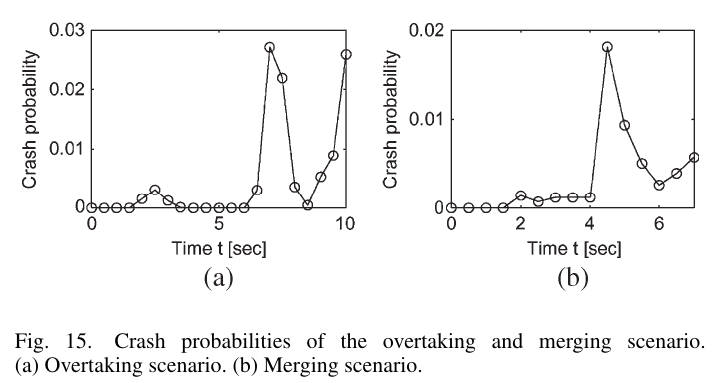
\includegraphics[width=0.7\textwidth]{img/35}\label{fig:35}
            \end{subfigure}
        \end{figure}
        \clearpage
        
        \hline
        \noindent \textbf{Referencia:}~\cite{pavel2022vision}                                          \\
        \textbf{Título:}                                                                               \\
        Vision-based autonomous vehicle systems based on deep learning: A systematic literature review \\
        \textbf{Autores:}
        Pavel, Monirul Islam and Tan, Siok Yee and Abdullah, Azizi                                     \\
        \textbf{Año:}
        2022                                                                                           \\
        \textbf{Revista:}
        Applied Sciences                                                                               \\
        \textbf{URL:}
        \url{https://www.mdpi.com/2076-3417/12/14/6831}                                                \\
        \textbf{Resumen:}                                                                              \\
        \begin{itemize}
            \item Durante la última década, los sistemas de vehículos autónomos (AVS) han avanzado considerablemente debido a mejoras
            en la inteligencia artificial, con un impacto significativo en la seguridad vial y el futuro de los sistemas de transporte.
            \item Sin embargo, la producción a gran escala de AVS aún se enfrenta a desafíos debido al alto costo de la fusión
            de sensores y la falta de soluciones completas para abordar la incertidumbre en las carreteras.
            \item El artículo realiza una revisión sistemática de la literatura sobre el uso del aprendizaje profundo en AVS
            durante la última década.
            \item La revisión se divide en varios módulos que cubren diferentes aspectos, como análisis de percepción, toma de decisiones,
            control, planificación de trayectorias y visualización en sistemas de realidad aumentada tipo HUD.
            \item Se analizan investigaciones realizadas desde 2011 hasta 2021 que se centran en el uso de cámaras RGB como sensores principales.
            \item Se presta especial atención a los resultados finales, como la visualización en sistemas de realidad aumentada basados en HUD,
            que incluyen advertencias tempranas, marcadores en la carretera para mejorar la navegación y la seguridad al superponer información
            en vehículos y peatones en condiciones visuales extremas para reducir colisiones.
            \item La revisión destaca los métodos actuales de aprendizaje profundo que se basan únicamente en la visión de cámaras RGB
            en lugar de la compleja fusión de sensores.
            \item Se espera que este enfoque proporcione una vía para el desarrollo rápido de sistemas de vehículos autónomos prácticos,
            eficientes y seguros en términos de costos.
        \end{itemize}                                                                                  \\
        \begin{figure}[!ht]
            \begin{subfigure}
                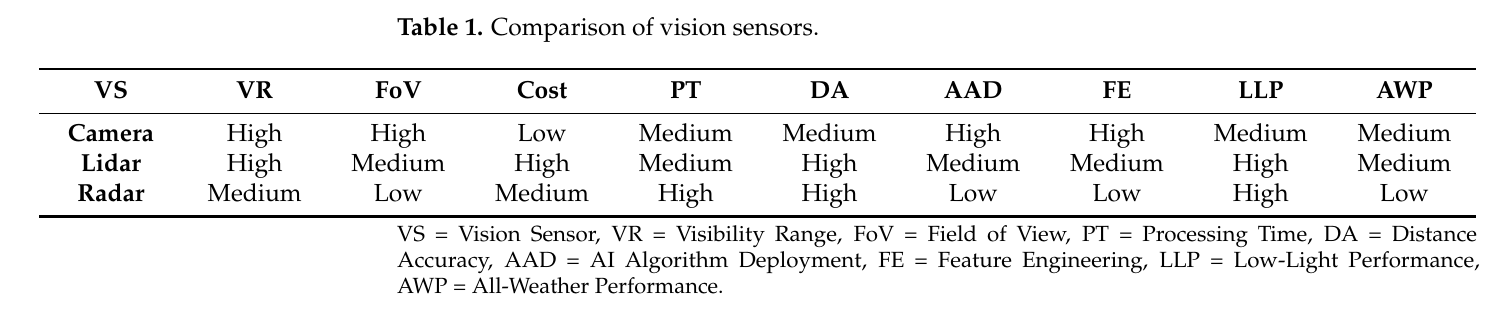
\includegraphics[width=1\textwidth]{img/71}\label{fig:71}
            \end{subfigure}
            \begin{subfigure}
                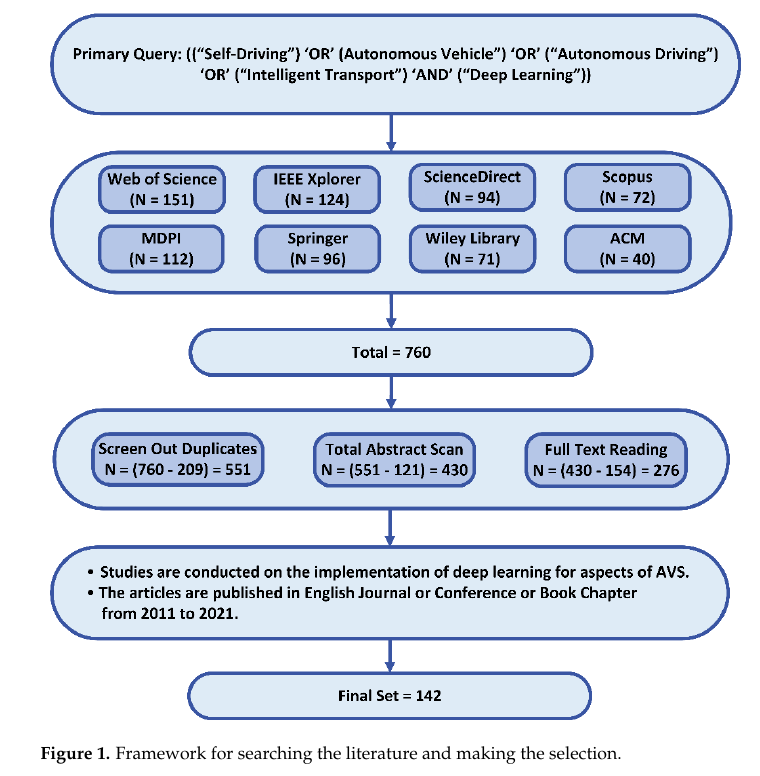
\includegraphics[width=0.5\textwidth]{img/72}\label{fig:72}
            \end{subfigure}
            \begin{subfigure}
                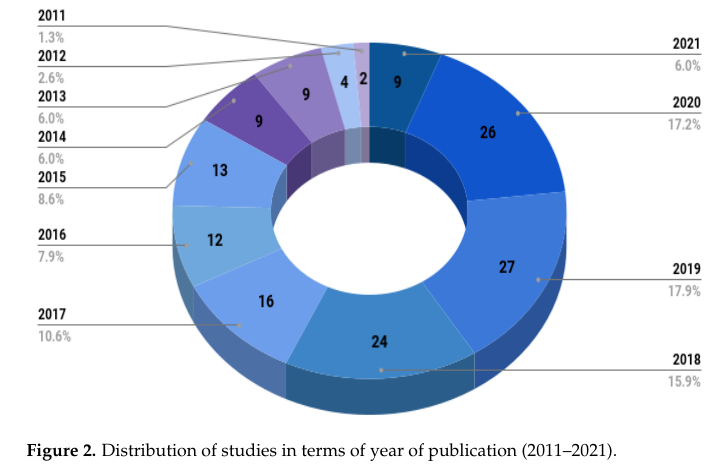
\includegraphics[width=0.6\textwidth]{img/73}\label{fig:73}
            \end{subfigure}
            \begin{subfigure}
                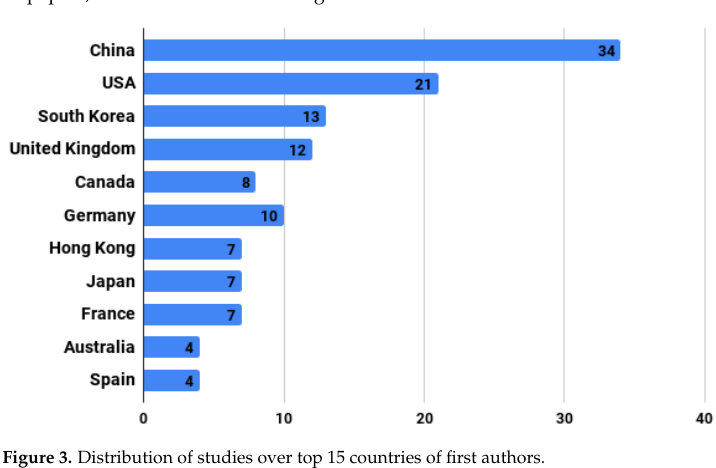
\includegraphics[width=0.5\textwidth]{img/74}\label{fig:74}
            \end{subfigure}
        \end{figure}
        \begin{figure}[!ht]
            \begin{subfigure}
                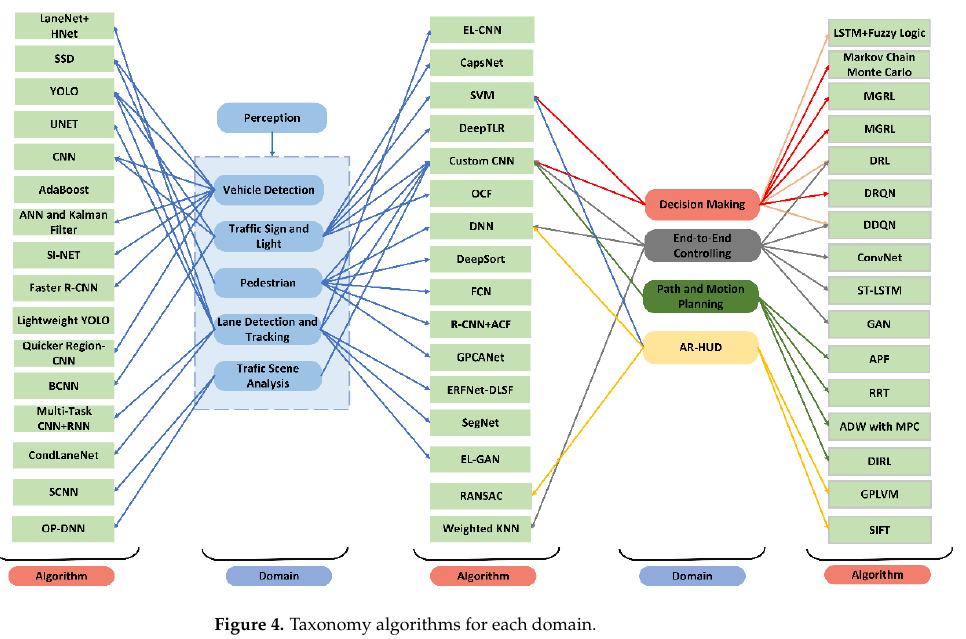
\includegraphics[width=1\textwidth]{img/75}\label{fig:75}
            \end{subfigure}
            \begin{subfigure}
                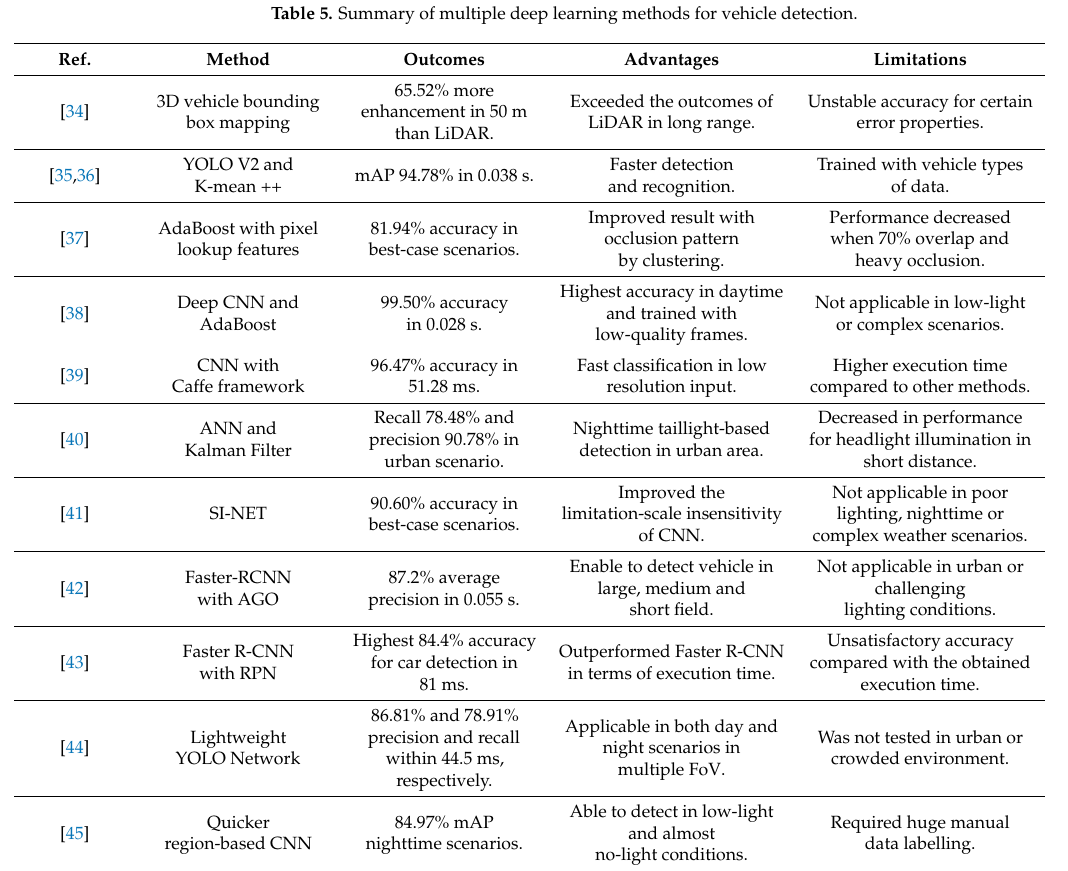
\includegraphics[width=1\textwidth]{img/76}\label{fig:76}
            \end{subfigure}
        \end{figure}
        \clearpage
        
        \hline
        \noindent \textbf{Referencia:}~\cite{alam2022cost}                                             \\
        \textbf{Título:}                                                                               \\
        A cost-effective computer vision-based vehicle detection system                                \\
        \textbf{Autores:}
        Alam, Altaf and Jaffery, Zainul Abdin and Sharma, Himanshu                                     \\
        \textbf{Año:}
        2022                                                                                           \\
        \textbf{Revista:}
        Concurrent Engineering                                                                         \\
        \textbf{URL:}
        \url{https://journals.sagepub.com/doi/abs/10.1177/1063293X211069193}                           \\
        \textbf{Resumen:}                                                                              \\
        \begin{itemize}
            \item El artículo se centra en la detección de vehículos, una parte crucial en el desarrollo de sistemas de conducción autónoma.
            \item Destaca la importancia del procesamiento rápido y la detección precisa de vehículos en un sistema de detección autónoma.
            \item Propone un sistema de detección de vehículos basado en visión por computadora que utiliza un algoritmo
            de Gentle Adaptive Boosting con características tipo Haar para generar hipótesis de vehículos de manera rápida.
            \item Para abordar este problema, se propone el uso de un algoritmo de Máquinas de Vectores de Soporte (SVM) entrenado con
            características del histograma de gradientes orientados (HOG) para filtrar las hipótesis falsas.
            \item El descriptor HOG utiliza la forma y los contornos de los vehículos, lo que mejora la precisión de la detección.
            \item Se combina el uso de características tipo Haar y características HOG para lograr los objetivos de detección en la conducción autónoma.
            \item El rendimiento del sistema propuesto se evalúa con imágenes capturadas tanto de día como de noche y se compara
            con tres detectores de vehículos existentes.
            \item Se observa que la precisión promedio del sistema propuesto es del 0.97 para imágenes capturadas de día
            y del 0.94 para imágenes capturadas de noche.
            \item Además, el sistema propuesto requiere 15 veces menos tiempo de entrenamiento en comparación con técnicas
            existentes para la misma cantidad de datos de imágenes y en la misma unidad de procesamiento central (CPU).
        \end{itemize}
        \begin{figure}[!ht]
            \begin{subfigure}
                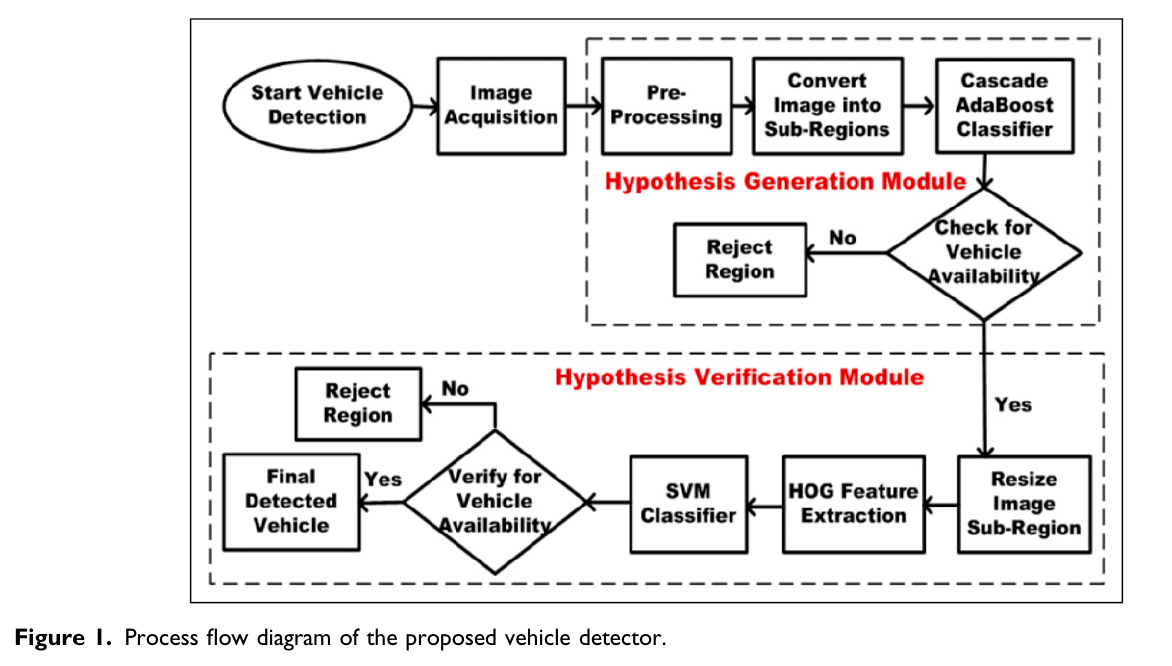
\includegraphics[width=0.5\textwidth]{img/81}\label{fig:81}
            \end{subfigure}
            \begin{subfigure}
                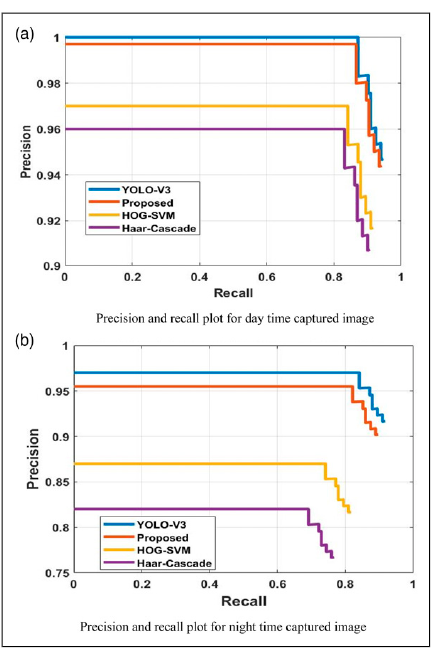
\includegraphics[width=0.5\textwidth]{img/86}\label{fig:82}
            \end{subfigure}
            \begin{subfigure}
                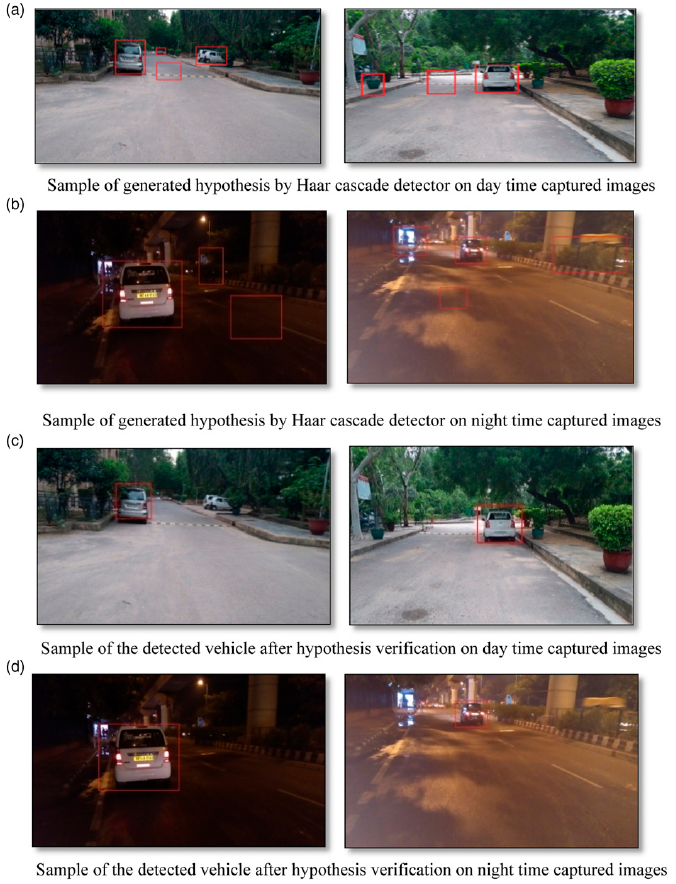
\includegraphics[width=0.5\textwidth]{img/84}\label{fig:84}
            \end{subfigure}
            \begin{subfigure}
                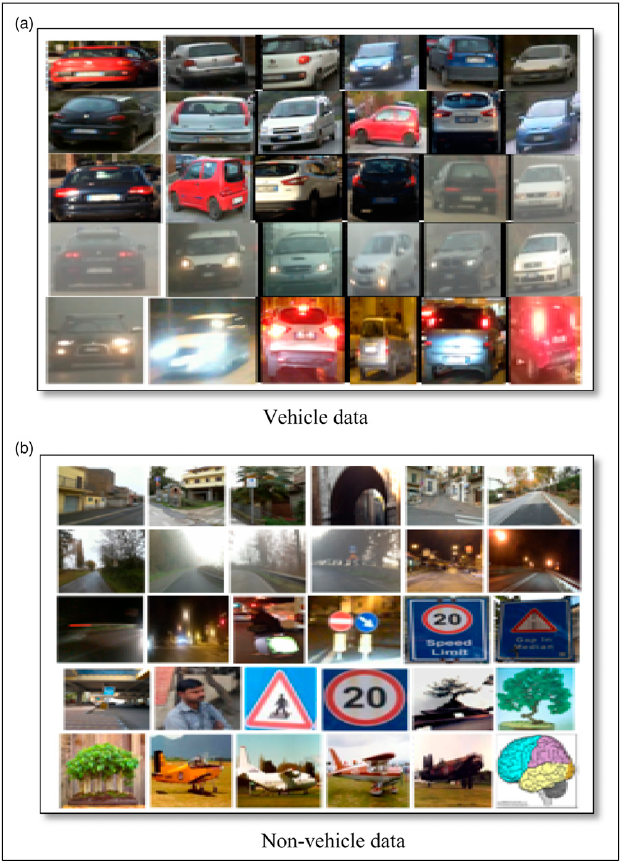
\includegraphics[width=0.5\textwidth]{img/82}\label{fig:86}
            \end{subfigure}
        \end{figure}
        \clearpage
    \end{longtable}
    \begin{table}
        \centering
        \caption{Tabla comparativa}
        \begin{tabular}{|p{4cm}|p{2cm}|p{2cm}|p{2cm}|p{2cm}|p{2cm}|}
            \hline
            \textbf{Características}
            & \textbf{Autonomous Driving Architectures \cite{bachute2021autonomous}}
            & \textbf{Vision-based Autonomous Car Racing \cite{cai2021vision}}
            & \textbf{Model-based Probabilistic Collision Detection \cite{althoff2009model}}
            & \textbf{Vision-based Autonomous Vehicle Systems \cite{pavel2022vision}}
            & \textbf{Cost-effective Vehicle Detection System \cite{alam2022cost}} \\
            \hline
            Uso de algoritmos de Aprendizaje Automático y Aprendizaje Profundo & X &   &   & X &   \\
            \hline
            Enfoque en la conducción autónoma                                  & X & X & X & X & X \\
            \hline
            Ventajas de la conducción autónoma                                 & X &   &   &   &   \\
            \hline
            Complejidad de los sistemas de conducción autónoma                 & X &   &   &   &   \\
            \hline
            Análisis de tareas en la conducción autónoma                       & X &   &   &   &   \\
            \hline
            Evaluación y comparación de algoritmos                             & X & X &   &   &   \\
            \hline
            Predicción estocástica de ocupación de la carretera                &   &   & X &   &   \\
            \hline
            Eficiencia en cálculos intensivos                                  &   & X & X &   &   \\
            \hline
            Utilización de cámaras RGB como sensores principales               &   & X &   & X &   \\
            \hline
            Detección de vehículos en conducción autónoma                      &   &   &   &   & X \\
            \hline
        \end{tabular}
    \end{table}
    \clearpage
    \section*{Metodología}
    \noindent La metodología propuesta se fundamenta en un enfoque iterativo que abarca diversas etapas para la implementación del sistema de detección
    y evasión de colisiones en vehículos autónomos. En primera instancia, se establecerá un entorno de simulación realista que refleje las condiciones de tráfico habituales.
    Posteriormente, se procederá a la adquisición y procesamiento de datos provenientes de los sensores de dicho entorno simulado. La fase siguiente implicará el diseño
    y la implementación de algoritmos de visión computacional para la detección temprana de eventos críticos en tiempo real. Estos algoritmos serán sometidos a un proceso
    de entrenamiento y ajuste utilizando técnicas de aprendizaje automático. Finalmente, se llevarán a cabo pruebas exhaustivas y evaluaciones para validar la efectividad
    y la precisión del sistema propuesto en situaciones simuladas de riesgo vial.
    \section*{Calendario de actividades}
    \begin{table}[htbp]
        \centering
        \caption{Calendario de Actividades}
        \begin{tabular}{|>{\raggedright\arraybackslash}p{4cm}|p{6cm}|p{3cm}|}
            \hline
            \textbf{Actividad}                          & \textbf{Descripción}                                        & \textbf{Duración} \\ \hline
            Investigación Preliminar                    & Revisión bibliográfica y análisis de entornos de simulación & 2 meses \\ \hline
            Diseño y Configuración del Entorno Simulado & Configuración del entorno y modelos de comportamiento & 1 mes \\ \hline
            Adquisición y Procesamiento de Datos        & Recopilación y procesamiento de datos de sensores & 3 meses \\ \hline
            Desarrollo y Entrenamiento de Algoritmos    & Implementación y entrenamiento de algoritmos de detección & 4 meses \\ \hline
            Evaluación y Ajuste del Sistema             & Pruebas exhaustivas y ajustes del sistema                   & 2 meses           \\ \hline
            Documentación y Análisis de Resultados      & Documentación y análisis crítico de resultados & 1 mes \\ \hline
            Redacción y Presentación de la Tesis        & Redacción y preparación para defensa oral                   & 1 mes             \\ \hline
        \end{tabular}
    \end{table}
    \clearpage
    \section*{Referencias bibliográficas}
    \bibliographystyle{acm}
    \bibliography{referecias}
\end{document}
